%%%%%%%%%%%%%%%%%%%%%%%%%%%%%%%%%%%%%%%%%%%%%%%%%%%%%%%%%%%%%%%%%%%%%%%%%%%%
%%%%%%%%%%%%%%%%%%%%%%%%%%%%%%%%%%%%%%%%%%%%%%%%%%%%%%%%%%%%%%%%%%%%%%%%%%%%
% Article
%%%%%%%%%%%%%%%%%%%%%%%%%%%%%%%%%%%%%%%%%%%%%%%%%%%%%%%%%%%%%%%%%%%%%%%%%%%%
%%%%%%%%%%%%%%%%%%%%%%%%%%%%%%%%%%%%%%%%%%%%%%%%%%%%%%%%%%%%%%%%%%%%%%%%%%%%
% Unesp
%%%%%%%%%%%%%%%%%%%%%%%%%%%%%%%%%%%%%%%%%%%%%%%%%%%%%%%%%%%%%%%%%%%%%%%%%%%%
%%%%%%%%%%%%%%%%%%%%%%%%%%%%%%%%%%%%%%%%%%%%%%%%%%%%%%%%%%%%%%%%%%%%%%%%%%%%
\documentclass[a4paper,times,12pt]{article}
\usepackage{amsthm}
\usepackage[figuresright]{rotating}
\usepackage{graphicx}
\usepackage{booktabs}
\graphicspath{ {./images/} }
\usepackage{amssymb}
\usepackage{graphicx}
\usepackage{fancybox}
\usepackage{amsmath}
\usepackage{picinpar}
\usepackage{colortbl}
\usepackage{wasysym}
\usepackage{txfonts}
\usepackage{pb-diagram}
\usepackage{relsize}
\usepackage{tikz}
\usepackage{pgfplots}
\usepackage{subfigure}
\usepackage{algorithm}
\usepackage{algorithmic}
\usepackage{geometry}
\pgfplotsset{compat=1.18}

\geometry{
  a4paper,         % Tamanho do papel
  left=2.5cm,      % Margem esquerda
  right=2.5cm,     % Margem direita
  top=2.5cm,         % Margem superior
  bottom=2.5cm       % Margem inferior
}

\begin{document}
\begin{titlepage}
	\begin{center}
	
	%\begin{figure}[!ht]
	%\centering
	%\includegraphics[width=2cm]{c:/ufba.jpg}
	%\end{figure}

		\Huge{Instituto de Bioci\^{e}ncias, Letras e Ci\^{e}ncias Exatas, Unesp}\\
		\large{Departamento de Ciência da Computação e Estatística}\\ 
		
		\vspace{15pt}
        \vspace{95pt}
        \textbf{\LARGE{Apple M-Series}}\\
		%\title{{\large{Título}}}
		\vspace{3,5cm}
        Carlos Eduardo Nogueiro Silva\\
        Felipe Gomes da Silva \\
        Renan Sinhorini Pimentel \\
	\end{center}
	
	
	\vspace{1cm}
	\begin{center}
		\vspace{\fill}
		 Novembro\\
		 2024
			\end{center}
\end{titlepage}
%%%%%%%%%%%%%%%%%%%%%%%%%%%%%%%%%%%%%%%%%%%%%%%%%%%%%%%%%%%%%%%%%%%%%%%%%%%%%
%%%%%%%%%%%%%%%%%%%%%%%%%%%%%%%%%%%%%%%%%%%%%%%%%%%%%%%%%%%%%%%%%%%%%%%%%%%%%
\newpage
\tableofcontents
\thispagestyle{empty}
\newpage
\section{Introdução}
\hspace*{+15pt} 
A série de processadores \textbf{Apple M} representa uma mudança decisiva na estratégia corporativa de design e produção de chips, definindo uma nova era de autonomia tecnológica e otimização integral. Desde que a Apple iniciou, em 2020, sua transição dos processadores x86-64 para chips próprios baseados em arquitetura ARM, a empresa abriu caminho para uma arquitetura que une alta eficiência energética a um desempenho robusto e escalável \cite{apple_silicon_overview}. Com esse movimento, deixou de depender de terceiros, como a Intel, para priorizar um controle total sobre o hardware que equipa seus dispositivos, aprimorando ainda mais a integração e a otimização que já caracterizavam os processadores da série A em dispositivos móveis.

Embora o início do desenvolvimento desses processadores ainda seja incerto, sabe-se que ele se apoiou em décadas de avanços na arquitetura e organização de computadores. Neste artigo, exploraremos a história, os desafios e as inovações por trás da arquitetura dos processadores da série M, analisando tanto a evolução técnica quanto o impacto significativo dessa tecnologia no mercado de dispositivos comerciais e no desempenho de alto nível. Nossa análise busca oferecer uma perspectiva que combina uma visão geral abrangente com uma avaliação aprofundada da arquitetura ARM, destacando como a Apple Silicon se posiciona como um marco na computação moderna.

\section{História}
\hspace{+15pt} 
A série M de chips da Apple representa uma mudança significativa na arquitetura dos computadores Mac, iniciada com o M1 em 2020. Não obstante, esta série de processadores também representa a excelência em toda a área comercial de arquitetura de computadores. Esses processadores, baseado em ARM, foi projetado para integrar CPU, GPU e memória unificada, permitindo eficiência energética e desempenho sem precedentes. Em 2021, a Apple lançou os M1 Pro e M1 Max, aprimorando essas capacidades com maior largura de banda de memória, mais núcleos de processamento e melhorias em gráficos, voltados para profissionais que exigem alto desempenho em aplicações gráficas e científicas.
\subsection{Primeira Geração: Apple M1}
\hspace{+15pt} 
O primeiro processador da série, o M1, foi lançado em novembro de 2020. Esse SoC (System on a Chip) foi baseado na arquitetura ARM, tradicionalmente usada em dispositivos móveis, e incluía uma CPU de oito núcleos e uma GPU integrada com até oito núcleos. O M1 se destacou por sua eficiência energética, ao mesmo tempo que oferecia um desempenho impressionante, permitindo à Apple melhorar a autonomia de seus laptops e reduzir a dissipação de calor. Com o M1, a Apple também introduziu uma arquitetura de memória unificada, na qual CPU, GPU e outros componentes compartilham a mesma memória, o que reduz a latência e aumenta a eficiência.
Em 2021, a Apple expandiu a linha M1 com os modelos M1 Pro e M1 Max, que ofereceram melhorias substanciais em termos de capacidade de processamento e memória. Esses chips, voltados para profissionais, trouxeram GPUs mais poderosas, suportando tarefas complexas de edição de vídeo e renderização gráfica. Em 2022, a Apple revelou o M1 Ultra, combinando dois M1 Max em um único chip, usando uma interconexão chamada UltraFusion, com desempenho similar ao de estações de trabalho, reforçando o compromisso da Apple com a escalabilidade e a modularidade de sua arquitetura própria.

\subsection{Segunda Geração: Apple M2}
\hspace{+15pt} 
Em junho de 2022, a Apple apresentou o M2, uma atualização que oferecia desempenho até 18\% superior ao M1, com uma GPU aprimorada e um aumento na largura de banda da memória. A série M2 continuou a tradição de alta eficiência energética, enquanto introduzia avanços em aprendizado de máquina e IA. A Apple também lançou variantes do M2, como o M2 Pro e o M2 Max, que oferecem desempenho gráfico superior e são projetados para aplicativos que exigem processamento gráfico intenso
\subsection{Terceira Geração: Apple M3}
\hspace{+15pt}
Lançado em outubro de 2023, o M3 é o primeiro processador da série M fabricado com o processo de 3 nm, trazendo melhorias significativas em desempenho e eficiência energética. Este chip é capaz de executar tarefas complexas, como ray tracing em tempo real, graças ao aumento de núcleos tanto na CPU quanto na GPU. A Apple também lançou versões avançadas do M3, o M3 Pro e o M3 Max, que incluem até 16 núcleos de CPU e 40 núcleos de GPU, com capacidades de memória RAM que chegam a 128 GB, tornando-os ideais para cargas de trabalho avançadas e uso profissional.

Esse avanço é uma parte essencial da estratégia da Apple para ter controle total sobre o hardware e o software de seus dispositivos, otimizando o desempenho para suas necessidades específicas, como maior duração da bateria e melhor desempenho em tarefas gráficas e de IA. 

Vale a consideração de que estes processadores só puderam ser desenvolvidos devido devido à arquitetura ARM e o Conjunto Reduzido de Instruções (RISC), tópicos que abordaremos no próximo capítulo.

\begin{figure}[ht]
    \centering
    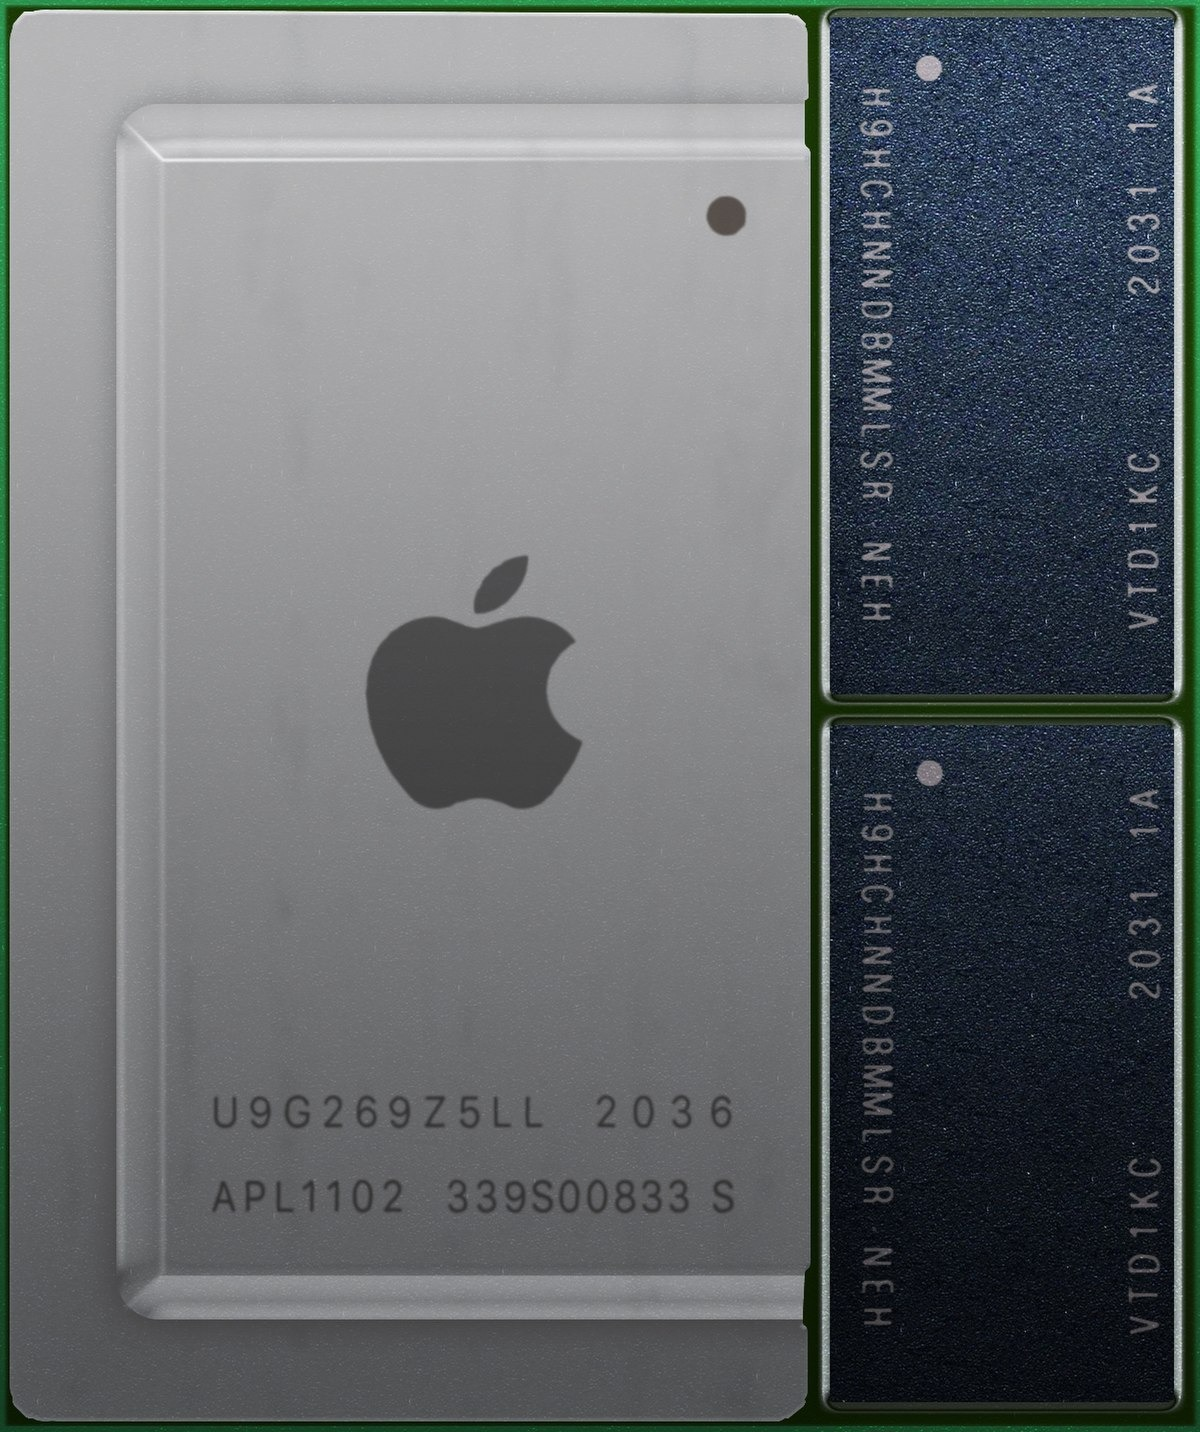
\includegraphics[width=0.8\textwidth]{./apple.jpeg}
    \caption{Chip M1}
    \label{fig:apple_m1}
\end{figure}


\section{Arquitetura ARM}
\hspace{+15pt}
A arquitetura ARM (para Advanced RISC Machines), é uma das principais arquiteturas baseadas no modelo de Conjunto Reduzido de Instruções (RISC), projetada para otimizar eficiência energética e desempenho. Desenvolvida inicialmente na década de 1980, a arquitetura ARM evoluiu para atender a necessidades de baixo consumo energético e alta eficiência em sistemas embarcados e dispositivos móveis.

A filosofia RISC, na qual a ARM se fundamenta, propõe um conjunto de instruções simplificadas em comparação com arquiteturas de Conjunto Complexo de Instruções (CISC), como a arquitetura x86. Esse conjunto reduzido permite que cada instrução seja executada em um ciclo de clock, aumentando a eficiência do pipeline e possibilitando operações mais rápidas com menor dissipação de energia. De acordo com Hennessy e Patterson (2017), o design RISC é particularmente eficaz em tarefas que requerem alto throughput, já que uma instrução de ciclo único facilita o empilhamento de múltiplas operações em paralelo.

Em termos técnicos, a arquitetura ARM apresenta características de um pipeline profundo e previsível, com múltiplos estágios para decodificação e execução das instruções, o que aumenta a velocidade de processamento e a previsibilidade do desempenho. Além disso, as versões mais recentes da arquitetura ARM, como a ARMv8 e ARMv9, introduzem suporte a instruções de 64 bits, aumentando a capacidade de endereçamento de memória e permitindo um maior desempenho em sistemas operacionais modernos e aplicações que exigem grandes volumes de dados. Em específico, abordaremos detalhes das aplicações da arquitetura ARM dentro da série de processadores M da Apple, destacando como a combinação de eficiência energética e desempenho robusto tem sido fundamental para a evolução desses chips e o impacto que eles têm tido no mercado de dispositivos comerciais e de alto desempenho.

\newpage
\section{Arquitetura e Organização}
\hspace{+15pt} A série de chips M da Apple representa uma das arquiteturas de System-on-a-Chip (SoC) mais avançadas no mercado. Esses chips integram múltiplos componentes, como CPU, GPU, memória e unidades de processamento neural, em um único chip de silício, permitindo maior eficiência energética e uma integração mais profunda entre os componentes do hardware e o software.

Os chips da série M possuem um grande número de transistores, com o M1 contando com 16 bilhões, sendo capaz de fazer até 11 trilhões de operações por segundo. Além disso, a GPU integrada nesses chips conta com 8 núcleos no M1 e 32 núcleos no M1 Max, permitindo um processamento gráfico robusto sem a necessidade de uma GPU dedicada. Mas atualmente, com o chip M3, a Apple deu mais um salto significativo em termos de potência e eficiência, trazendo uma quantidade ainda maior de transistores, ultrapassando os 25 bilhões, o que permite uma capacidade de processamento ainda mais avançada e otimizada para tarefas intensivas de cálculo. Além disso, a GPU integrada no M3 também foi aprimorada, contando com até 40 núcleos em sua versão mais poderosa, oferecendo desempenho gráfico excepcional.

\subsection{Núcleos}
\hspace{+15pt}
Os chips da série M empregam uma arquitetura heterogênea de múltiplos núcleos - uma abordagem inspirada na arquitetura ARM big.LITTLE - combinando núcleos de alto desempenho (Firestorm) e núcleos de alta eficiência (Icestorm). Essa combinação permite que o sistema ajuste seu consumo energético com base na tarefa em execução, dando preferência para núcleos de alto desempenho em tarefas intensivas, enquanto, para operações mais leves, núcleos de alta eficiência energética são usados. 


\subsection{Memória}
\hspace{+15pt}
Uma das inovações fundamentais dessa arquitetura é o conceito de memória unificada. Diferente dos designs tradicionais, nos quais CPU e GPU utilizam memórias separadas, a arquitetura dos chips M permite que todos os processadores acessem a mesma memória física. Isso reduz a necessidade de cópias redundantes de dados e melhora a comunicação entre CPU e GPU, resultando em um desempenho mais eficiente e menores tempos de resposta. Tal memória unificada também conta com uma largura de banda de 68.25 GB/s para o processador M1, podendo chegar até 400 GB/s para o M1 Max. Podemos observar a disposição da memória na figura [\ref{fig:apple_m1_ultra}].

\begin{figure}[ht]
    \centering
    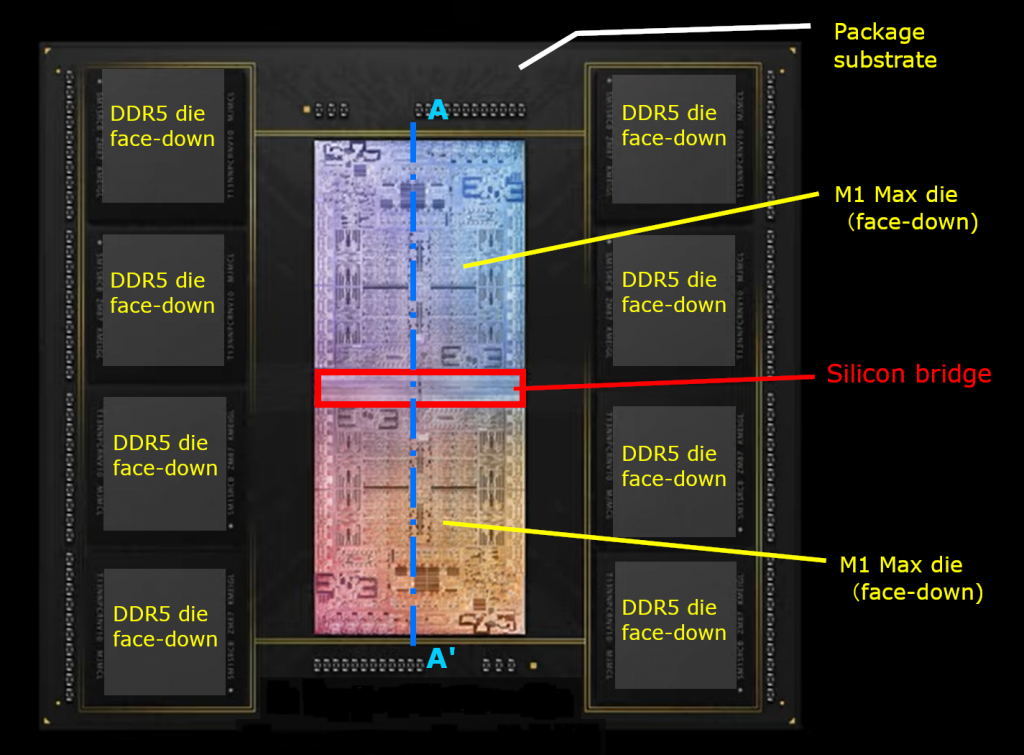
\includegraphics[width=0.9\textwidth]{./apple-m1-ultra.png}
    \caption{Apple M1 Ultra}
    \label{fig:apple_m1_ultra}
\end{figure}

\newpage
\section{Desempenho}
\hspace{+15pt}
A série M da Apple Silicon, devido a sua eficiência energética, alto desempenho e arquitetura \textit{System on a Chip (SoC)}, revolucionou o mercado. O processador \textbf{M1} e seus sucessores trouxeram avanços significativos quando comparados a processadores baseados na arquitetura x86 e similares usados em notebooks.

\subsection{Apple M1 vs Intel (x86)}
\hspace{+15pt}
O \textit{SoC} Apple M1 trouxe uma mudança de paradigmo no setor de processadores na época de seu lançamente ao superar diversos processador x86 da Intel, antes usados em dispositivos da Apple, em especial na eficiência energética e gerenciamento de calor. construído baseado na arquitetura ARM, com oito núcleos divididos em quatro de alto desempenho e quatro de alta eficiência, o M1 foi capaz de superar laptops com Intel Core i7 e i9.

Uma das vantagens da série M é o uso de \textbf{memória unificada} em sua arquitetura, o que permite que processador e GPU entre outros componentesacessem a mesma pool de memória sem a necessidade de realizar a tranferência de dados entre os mesmos.\cite{apple_silicon_potential} Esse design melhora significativamente o desempenho em algoritmos que envolvam grande movimentação de dados.\cite{apple_m_vs_intel}

\subsection{Apple M2: A Evolução do M1}
\hspace{+15pt}
O lançamento do \textbf{M2}, Apple foi capaz de aumentar ainda mais a eficiência e poder de processamento de sua linha de chips. O M2 apresentou um aumento de 40\% em desempenho quando comparado com o seu antecessor M1, possuindo mais núcleos dedidcados à \textbf{GPU (Graphics Processing Unit)} e a \textbf{NPU (Neural Processing Unit)}. Isso tornou, é claro, os notebooks que portavam o M2 uma escolha mais robustas para ãplicações de aprendizado de máquina, por exemplo \cite{usability_ml}. Estudos mostram que o M2 é altamente performático em tarefas de visão computacional e processamento de grande volumes de dados tabulares, chegando a até mesmo rivalizar com GPUs dedicadas da NVIDIA, especialmente em aplicações que não exigem precisão dupla, a qual a série M não possui. Mesmo com GPUs de alto desempenho como \textbf{RTX 3090} ou a \textbf{NVIDIA A100} mantendo a vantagem em certos domínios intensos computacionalmente, o \textbf{M2} se mostra uma esolha atraente para usuários comuns e pesquisadores.\cite{usability_ml}

\subsection{Desempenho em Computação Científica}
\hspace{+15pt}
O desempenho dos chips M da Apple também tem chamado a atenção na área de \textbf{computação científica}. Estudos comparativos mostraram que o \textbf{M1} e o \textbf{M1 Ultra} superam GPUs especialzada para computação de alto desempenho como a \textbf{NVIDIA V100} em uma série de benchmarks , especialmente em tarefas que se beneficiam de memória compartilhada entre CPU e GPU, eliminando os gargalos de transferência de dados. Nos benchmarks SHOC, que cobre características diferentes níveis, como a performance da arquitetura projeto, execução de algoritmos e aplicações reais de kernel, o \textbf{M1 Ultra} destacou-se significativamente em tarefas como multiplicação de matrizes e transformadas rápidas de Fourier, mantendo uma superioridade de até duas ordens de magnitude em relação às GPUs da NVIDIA em alguns testes \cite{apple_silicon_scientific_computing}.
Vale ressaltar que GPUs de alto desempenho podem consumir até 300W ou mais, o M1 e o M1 Ultra consomem entre 10W e 60W, uma diferença substancial.\cite{apple_silicon_scientific_computing}.

\subsection{Aplicações em Aprendizado de Máquina}
\hspace{+15pt}
Os chips \textbf{M1} e \textbf{M2} também têm se mostrado altamente eficazes para aplicações de \textbf{machine learning} e \textbf{deep learning}. Em tarefas que envolvem redes neurais convolucionais e processamento de linguagem natural, os dispositivos equipados com esses chips foram comparáveis, e muitas vezes superiores, a laptops com processadores Intel. Graças à \textbf{Neural Engine} dedicada, os chips M são capazes de acelerar significativamente o treinamento de modelos de aprendizado profundo, tornando-os uma excelente escolha para pesquisadores e profissionais que trabalham com aprendizado de máquina no dia a dia \cite{usability_ml, apple_silicon_potential}.

\section{Conclusão}
\hspace{+15pt}
A série Apple M redefine o que significa integrar hardware e software em um único propósito: criar dispositivos mais rápidos, inteligentes e eficientes. Não é apenas um avanço técnico; é uma declaração de como a inovação pode estar a serviço da experiência do usuário. Ao unificar processamento, gráficos e memória em uma arquitetura própria, a Apple reposiciona o conceito de eficiência no mercado de dispositivos, oferecendo mais que desempenho bruto – ela entrega uma sinergia completa, onde cada componente trabalha em função do outro, minimizando desperdícios e maximizando resultados.

Essa integração entre design de chip e software revela um caminho claro para o futuro: dispositivos onde o fluxo de dados é contínuo e otimizado, e onde cada operação ocorre sem atrito. Esse nível de controle sobre a arquitetura e o funcionamento dos chips não apenas transforma a experiência do usuário comum, mas também abre novas possibilidades para profissionais que exigem desempenho confiável e consistente. A série M não é apenas uma inovação incremental; é uma visão de como a tecnologia pode evoluir em um ciclo virtuoso de autonomia e aprimoramento, onde o desempenho se encontra com a eficiência, dando forma a um novo paradigma que influencia toda a indústria, além de redefinir o que esperamos dos dispositivos do futuro.


\newpage
\begin{thebibliography}{00}
\bibitem{brain_like_computing} Ou, W., Xiao, S., Zhu, C., Han, W., \& Zhang, Q. (2022). \textbf{An overview of brain-like computing: Architecture, applications, and future trends}. Frontiers in Neurorobotics, 16, 1041108.

\bibitem{apple_silicon_overview} Brown, M., \& Williams, J. (2022). \textbf{Apple Silicon: Powering the Future of Computing}. IEEE Xplore. Disponível em: https://ieeexplore.ieee.org/abstract/document/9926315.

\bibitem{apple_at_work} Apple Inc. (2021). \textbf{Apple at Work – M1 Overview}. Apple Business. Disponível em: https://www.apple.com/br/business/mac/pdf/Apple-at-Work-M1-Overview.pdf.

\bibitem{hardware_acceleration} Chen, Y., \& Li, X. (2021). \textbf{Hardware Acceleration Techniques for Next-Generation Computing}. In S. Kumar \& P. Jones (Eds.), Emerging Technologies in Computing (pp. 509-523). Springer, Cham. Disponível em: https://link.springer.com/chapter/10.1007/978-3-030-93677-8\_48

\bibitem{apple_m_vs_intel}
Vaibhav Dalakoti and Diptamon Chakraborty, ``Apple M1 Chip vs Intel (X86),'' \textit{EPRA International Journal of Research and Development}, vol. 7, no. 5, May 2022, doi: 10.36713/epra2016.

\bibitem{apple_silicon_potential}
Karol Struniawski, Aleksandra Konopka, and Ryszard Kozera, ``Exploring Apple Silicon's Potential from Simulation and Optimization Perspective,'' \textit{Institute of Information Technology, Warsaw University of Life Sciences}, 2024, doi: 10.1007/978-3-031-63775-9\_3.

\bibitem{usability_ml}
David Kasperek, Pawel Antonowicz, Marek Baranowski, Marta Sokolowska, and Michal Podpora, ``Comparison of the Usability of Apple M2 and M1 Processors for Various Machine Learning Tasks,'' \textit{Sensors}, vol. 23, no. 5424, June 2023, doi: 10.3390/s23125424.

\bibitem{apple_silicon_scientific_computing}
Connor Kenyon and Collin Capano, ``Apple Silicon Performance in Scientific Computing,'' \textit{Center for Scientific Computation and Data Science Research}, November 2022, arXiv:2211.00720.

\bibitem{Computer Architecture: A Quantitative Approach} 
Hennessy, J. L., \& Patterson, D. A. (2017). Computer Architecture: A Quantitative Approach. Morgan Kaufmann.
\end{thebibliography}
\end{document}

